\documentclass[12pt,journal]{IEEEtran}

\usepackage[utf8]{inputenc}
\usepackage{pgfplots}
\usepackage{caption}

\begin{document}

    \title{Lineal regression with one variable and one parameter for the cost
           function}
    \author{Alejandro Salgado G}
    \maketitle

    This problem consists in predicting differents ouputs based on some examples
    that the algorithm is going to receive. \\

    for example, we have the folowing points plotted in a graphic\\

    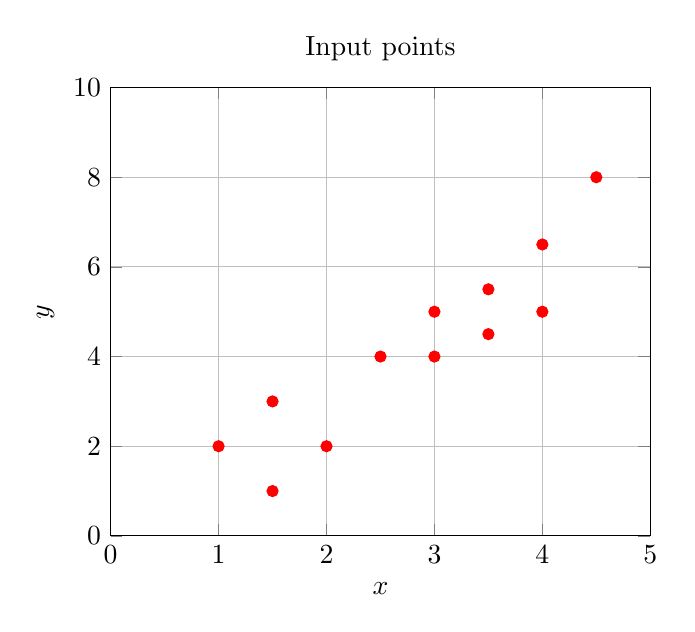
\begin{tikzpicture}
        \begin{axis}[
                      title={Input points},
                      xlabel=$x$,
                      ylabel=$y$,
                      xmin=0, xmax=5,
                      ymin=0, ymax=10,
                      grid=both
                    ]
            \addplot[color=red, only marks]
                coordinates{
                    (1,2)
                    (1.5,1)
                    (1.5,3)
                    (2,2)
                    (2.5,4)
                    (3,5)
                    (3,4)
                    (3.5,4.5)
                    (3.5,5.5)
                    (4,5)
                    (4,6.5)
                    (4.5,8)
                };
        \end{axis}
    \end{tikzpicture}

    What the algorithm will do is to draw a line as closser as posible to all
    the points in order to get the best aproximation posible to the original
    answers\\

    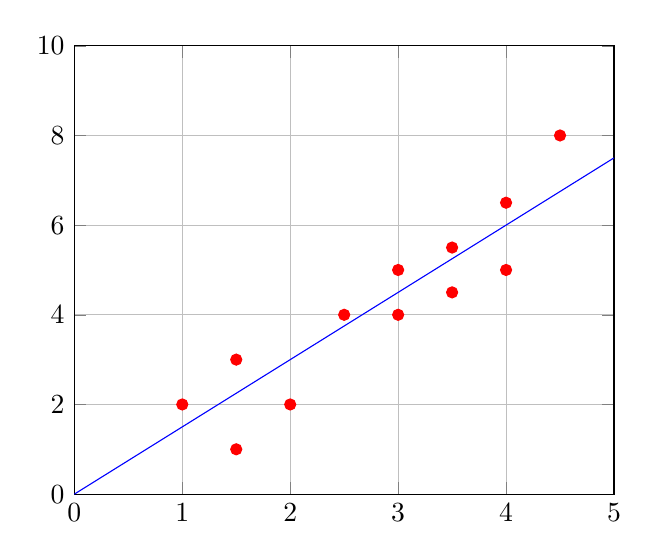
\begin{tikzpicture}
        \begin{axis}[
                      xmin=0, xmax=5,
                      ymin=0, ymax=10,
                      grid=both
                    ]
            \addplot[color=blue]{1.5*x};
            \addplot[color=red, only marks]
                coordinates{
                    (1,2)
                    (1.5,1)
                    (1.5,3)
                    (2,2)
                    (2.5,4)
                    (3,5)
                    (3,4)
                    (3.5,4.5)
                    (3.5,5.5)
                    (4,5)
                    (4,6.5)
                    (4.5,8)
                };

        \end{axis}
    \end{tikzpicture}

    When the right line is founded we can get an aproximatly answers to
    inputs, that not necesarly where given in first place, allowing to
    get more info from data.\\

    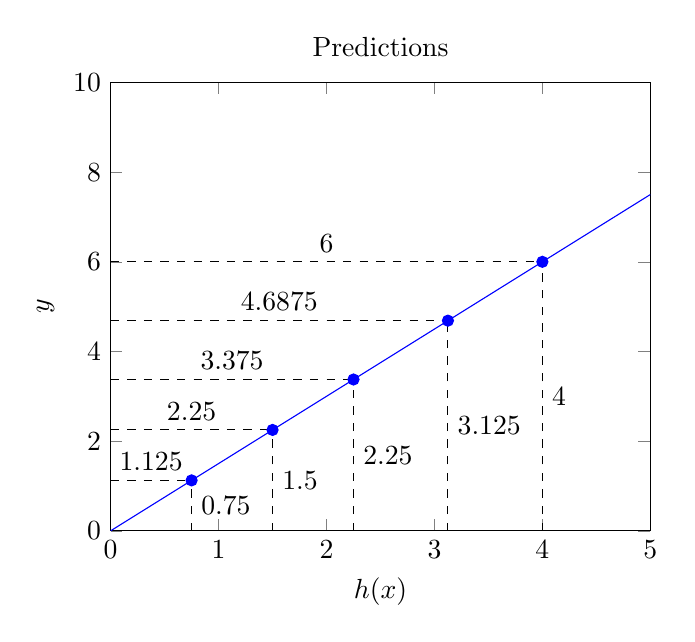
\begin{tikzpicture}
        \begin{axis}[
                      title={Predictions},
                      xlabel=$h(x)$,
                      ylabel=$y$,
                      xmin=0, xmax=5,
                      ymin=0, ymax=10,
                    ]
            \addplot[color=blue]{1.5*x};

            \draw[dashed] (axis cs: 0,1.125) -- node[above]{1.125} (axis cs: 0.75,1.125);
            \draw[dashed] (axis cs: 0.75,0) -- node[right]{0.75} (axis cs: 0.75,1.125);

            \draw[dashed] (axis cs: 0,2.25) -- node[above]{2.25} (axis cs: 1.5,2.25);
            \draw[dashed] (axis cs: 1.5,0) -- node[right]{1.5} (axis cs: 1.5,2.25);

            \draw[dashed] (axis cs: 0,3.375) -- node[above]{3.375} (axis cs: 2.25,3.375);
            \draw[dashed] (axis cs: 2.25,0) -- node[right]{2.25} (axis cs: 2.25,3.375);

            \draw[dashed] (axis cs: 0,4.6875) -- node[above]{4.6875} (axis cs: 3.125,4.6875);
            \draw[dashed] (axis cs: 3.125,0) -- node[right]{3.125} (axis cs: 3.125,4.6875);

            \draw[dashed] (axis cs: 0,6) -- node[above]{6} (axis cs: 4,6);
            \draw[dashed] (axis cs: 4,0) -- node[right]{4} (axis cs: 4,6);

            \addplot[color=blue, only marks]
                coordinates{
                    (0.75,1.125)
                    (1.5,2.25)
                    (2.25,3.375)
                    (3.125,4.6875)
                    (4,6)
                };

        \end{axis}
    \end{tikzpicture}

    In order to get this line we must define a function that give as the answers
    values, the functionwill be the equation of a line
    \begin{equation}
        h(x) = \theta_0 + \theta_1 x
    \end{equation}

    But taking into account that this is the first example that we are going to
    look at, we will eliminate the term that moves the graphic in the Y axis by
    make this variable equal to zero ($\theta_0 = 0$), this means  that the line
    that we will make will allways pass by the origin. In the next article this
    term will be used. In this article the function will be define as follow


    \begin{equation}
        h(x) = \theta x
    \end{equation}

    Now the problem will have two types of points: \\

    \begin{itemize}
        \item The result of the function $h(x)$
        \item The real result that we are going to call ($y$) \\
    \end{itemize}

    The next thing to do is compute how much the two sets of points differ, to
    do this we are going to use the cuadratic error of the two sets. Next we
    will give a practical example of how to get the formula. \\

    Lets say that in our problem we are going to have only three points to
    predict. Our function $h(x)$ gave the results $\{5,10,1\}$ and the correct
    results are $\{6,9,3\}$ and we want to cuantificate the error asocciated to
    this two answers.

    The first thing that must do is calculate the difference between this two
    sets:\\

    \begin{itemize}
        \item $5-6 = -1$
        \item $10-9 = 1$
        \item $1-3 = -2$ \\
    \end{itemize}

    The final result is another set $\{-1,1,-2\}$, this set contain positive and
    negative numbers, and if we decide to do the difference of the two sets in
    another order, for example results minus predictions, we will end up with a
    different set that can contain positive and negative numbers, as we only
    interested in calculate a number asociated to the error of our function
    $h(x)$ the negative numbers will not add any importat information, so we
    must eliminate this type of numbers in order to get only the information
    that we are interested on.

    To achive this gold we have two posible ways to do it, the first one is to
    add an absolute value to the calculation and the other is to squaring the
    results. The first option is not useful because later we will have to
    calculate a simple derivative to the resulting function and the absolute
    value is not derivable, this let us with the suquare option\\

    \begin{itemize}
        \item $(5-6)^2 = 1$
        \item $(10-9)^2 = 1$
        \item $(1-3)^2 = 4$\\
    \end{itemize}

    The result of this operation is the set $\{1,1,4\}$. Exelent, now we will
    never have a negative number in out resulting set, notice that our
    answers will be much bigger because we are using square of two as our
    method to eliminate the negative numbers, actually this doesn't metter
    because we are lookin for a number that describes the error associated to
    the prediction that we are computing so the range of the number is not too
    important.\\

    Now that we have our resulting set we want to get the mean of the errors,
    and this will be our error associated to the prediction that we have done\\

    \begin{itemize}
        \item $\frac{1+1+4}{3} = \frac{6}{3} = 2$ \\
    \end{itemize}

    Now that we have seen the process, we are gonig to formalize a little bit
    the process. The first thing that we are going to do is define a varible as
    the number of elements in each set \\

    \begin{itemize}
        \item $m = number\_of\_elements$ \\
    \end{itemize}

    Second we are going to define the resulting set as $\{x_1,x_2, ... , x_m\}$
    and the real resulting set as $\{y_1,y_2, ... , y_m\}$. This definition can
    be more concise because the first set is the result of the function $h(x)$,
    so we are going to define it as $h(x_i)$ and the second can be decribed as
    $y_i$.

    Now we will define the substration of each set as follows

    \begin{equation}
        h(x_i) - y_i \hspace{0.5cm} i=1, 2, ..., m
    \end{equation}

    Then adding the power of two part we will get the next expession

    \begin{equation}
        (h(x_i) - y_i)^2 \hspace{0.5cm} i=1, 2, ..., m
    \end{equation}

    Now adding the mean calculation we get

    \begin{equation}
        \frac{\sum_{i=1}^{m} (h(x_i) - y_i)^2}{m}
    \end{equation}

    Applying properties of sum

    \begin{equation}
       \frac{1}{m} \sum_{i=1}^{m} ( h(x_i) - y_i )^2
    \end{equation}

    Finally to make easier the future derivation we will add another term, a
    division by to, this step will be explained later.

    \begin{equation}
       \frac{1}{2m} \sum_{i=1}^{m} ( h(x_i) - y_i )^2
    \end{equation}

    This is the cuadratic error and will be used as our cost function in terms
    of the parameter $\theta$ to expess the error associated to the prediction
    of the algorithm with respect to the correct output that is given at the
    begin of the problem.

    \begin{equation}
       J(\theta) = \frac{1}{2m} \sum_{i=1}^{m} ( h(x_i) - y_i )^2
    \end{equation}

    This equation will have the following graphic

    \begin{figure}[h!]
        \begin{tikzpicture}
            \begin{axis}[
                         title={Cost function},
                         xlabel=$\theta$,
                         ylabel=$J(\theta)$,
                         ymin=0, ymax=25,
                         xtick=\empty,
                         ytick=\empty
                        ]
                \addplot[mark=none, color=blue]{x^2};
            \end{axis}
        \end{tikzpicture}
    \end{figure}

    The next step is define a way to make the error as small as posible,
    to do this we will use a famus algorithm called gradient decend.
    the formula of the algorithm is show bellow

    \begin{equation}
        \theta := \theta - \alpha
            \Bigg(
                \frac{d}{d \theta} J(\theta)
            \Bigg)
    \end{equation}

    The objective of this function is to actualize the parameter $\theta$
    of the cost function J minimizing the error in each iteration, this
    is done by searching the path to the global minimum.

    for those of you who are not familiar with the derivarives, is highly
    recomendable to look at the Derivative fundamentals article that is in
    located in the documentation directory.\\

    Now lets analyze the formula, the fist simbol is the $\theta$ that is the
    parameter of the cost function, the second is the $:=$ which means assign,
    this make sence because we are trying to update the parameter of the
    function trying to make it as closer to the minimum as possible.

    \begin{figure}[ht!]
        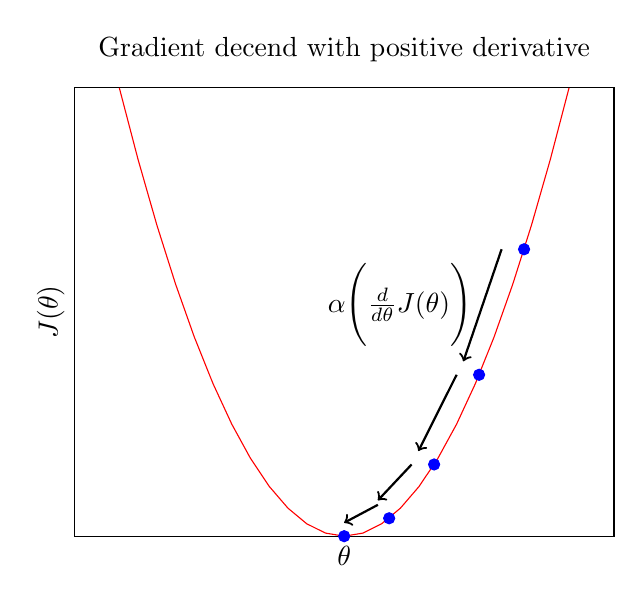
\begin{tikzpicture}
            \begin{axis}[
                         title={Gradient decend with positive derivative},
                         xlabel=$\theta$,
                         ylabel=$J(\theta)$,
                         ymin=0, ymax=25,
                         xtick=\empty,
                         ytick=\empty
                        ]
                \addplot[mark=none, color=red]{x^2};

                \draw[thick,->] (axis cs: 3.5,16) -- node[left]{$\alpha \Bigg(\frac{d}{d \theta} J(\theta)\Bigg)$} (axis cs: 2.65,9.75);
                \draw[thick,->] (axis cs: 2.5,9) -- (axis cs: 1.65,4.75);
                \draw[thick,->] (axis cs: 1.5,4) -- (axis cs: 0.75,2);
                \draw[thick,->] (axis cs: 0.75,1.75) -- (axis cs: 0,0.75);

                \addplot[color=blue, only marks]
                coordinates{
                    (4,16)
                    (3,9)
                    (2,4)
                    (1,1)
                    (0,0)
                };
            \end{axis}
        \end{tikzpicture}
    \end{figure}

    \begin{figure}[ht!]
        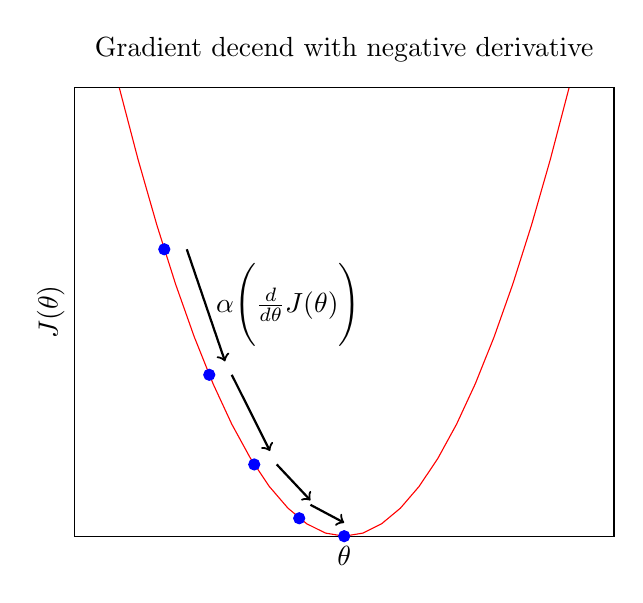
\begin{tikzpicture}
            \begin{axis}[
                         title={Gradient decend with negative derivative},
                         xlabel=$\theta$,
                         ylabel=$J(\theta)$,
                         ymin=0, ymax=25,
                         xtick=\empty,
                         ytick=\empty
                        ]
                \addplot[mark=none, color=red]{x^2};

                \draw[thick,->] (axis cs: -3.5,16) -- node[right]{$\alpha\Bigg(\frac{d}{d\theta}J(\theta)\Bigg)$} (axis cs: -2.65,9.75);
                \draw[thick,->] (axis cs: -2.5,9) -- (axis cs: -1.65,4.75);
                \draw[thick,->] (axis cs: -1.5,4) -- (axis cs: -0.75,2);
                \draw[thick,->] (axis cs: -0.75,1.75) -- (axis cs: -0,0.75);

                \addplot[color=blue, only marks]
                coordinates{
                    (-4,16)
                    (-3,9)
                    (-2,4)
                    (-1,1)
                    (0,0)
                };
            \end{axis}
        \end{tikzpicture}
    \end{figure}

    \vspace{8cm}

    Now the first thing to do in order to use the gradient desent in our cost
    function is replace the function $J(\theta)$ in the formula

    \begin{equation}
        \theta := \theta - \alpha
            \Bigg(
                \frac{d}{d \theta}
                    \Bigg[
                        \frac{1}{2m} \sum_{i=1}^{m} ( h(x_i) - y_i )^2
                    \Bigg]
            \Bigg)
    \end{equation}

    Now the factor of the denominator has no influence on the function so it
    can be tranlated outside of the derivative

    \begin{equation}
        \theta := \theta - \alpha \frac{1}{2m}
            \Bigg(
                \frac{d}{d \theta}
                    \Bigg[
                        \sum_{i=1}^{m} (\theta x_i - y_i)^2
                    \Bigg]
            \Bigg)
    \end{equation}

    The derivative of the summatory is equal to the derivative of each term and
    then add each result, so we can insert the dirivative into the summary

    \begin{equation}
        \theta := \theta - \alpha
            \Bigg(
                \frac{1}{2m} \sum_{i=1}^{m}
                    \Bigg[
                        \frac{d}{d \theta} (\theta x_i - y_i)^2
                    \Bigg]
            \Bigg)
    \end{equation}

    Then we calculate the derivative, notice that because of derivative
    properties we must calculate the outside derivative multiplied by the inside
    derivative

    \begin{equation}
        \theta := \theta - \alpha
            \Bigg(
                \frac{1}{2m} \sum_{i=1}^{m}
                    \Bigg[
                        2(\theta x_i - y_i) \frac{d}{d \theta}(\theta x_i - y_i)
                    \Bigg]
            \Bigg)
    \end{equation}

    Now we calculate the inside derivative

    \begin{equation}
        \theta := \theta - \alpha
            \Bigg(
                \frac{1}{2m} \sum_{i=1}^{m}
                    \Big[
                        2 (\theta x_i - y_i) (x_i - 0)
                    \Big]
            \Bigg)
    \end{equation}

    Now we can take the factor 2 outside the summatory

    \begin{equation}
        \theta := \theta - \alpha
            \Bigg(
                \frac{2}{2m} \sum_{i=1}^{m}
                    \Big[
                        (\theta x_i - y_i) x_i
                    \Big]
            \Bigg)
    \end{equation}

    Finally we can see the reason why the denominator has a extra factor
    (the 2 that we added at the begining), this is with the objective
    to cancel the 2 in the numerator that result of the derivative. Finaly
    this is the resulting function that we are going to use to minimize the
    error of the algorithm

    \begin{equation}
        \theta := \theta - \alpha
            \Bigg(
                \frac{1}{m} \sum_{i=1}^{m}
                    \Big[
                        (\theta x_i - y_i) x_i
                    \Big]
            \Bigg)
    \end{equation}

\end{document}
